% Template Author: Clara Eleonore Pavillet
% Version: 1.0
% This work is licensed under a Creative Commons Attribution 4.0 International License.

\documentclass[12pt, a4paper]{report}
\usepackage[utf8]{inputenc} %utf8 codierung

\usepackage{amsmath, amssymb,amsfonts} %AMS math packets
\usepackage{graphicx} %For pictures

\usepackage{datetime} %For dates

\usepackage[usenames,dvipsnames]{xcolor} %For coloring text and equations

\usepackage[bookmarks,colorlinks=true]{hyperref} %For referencing
\hypersetup{
	colorlinks,
	linktocpage,
	citecolor=black,
	filecolor=black,
	linkcolor=black,
	urlcolor=black
}
\numberwithin{equation}{section} % Section prefix for equation names

\usepackage{siunitx} %For units

\usepackage[section]{placeins} %Floats nicht über section Grenze, \FloatBarrier baut grenze 

\usepackage{pgfplots}
%\DeclareUnicodeCharacter{2212}{-}
\usepgfplotslibrary{groupplots, dateplot}
\usetikzlibrary{external, patterns, shapes.arrows, decorations.pathreplacing,calligraphy}
\pgfplotsset{compat=newest}
\usepackage[figure]{hypcap} %Links auf abbildungen springen auf das bild statt auf die caption - muss nach hyperref eingebunden werden, \capstart definiert sprungpunkt, bei [figure] kommt automatisch einer


%Für doppelten unterstrich:
\newcommand{\matrixvariable}[1]{\underline{\underline{\boldsymbol{\mathit{#1}}}}} 

%Für bilder \img{dateiname}{breite}{caption}{label}
\newcommand{\img}[4]{
	\begin{figure}
		\centering
		\includegraphics[width = #2]{#1}
		\caption{#3}
		\label{#4}
	\end{figure}
}
%Für tex.bilder \inp{dateiname}{caption}{label}
\newcommand{\inp}[3]{
	\begin{figure}
		\centering
		\input{#1}
		\caption{#2}
		\label{#3}
	\end{figure}
}
%für totale Ableitung
\newcommand{\tAbl}[2]{\frac{\mathrm{d}#1}{\mathrm{d}#2}}
%für partielle Ableitung
\newcommand{\pAbl}[2]{\frac{\partial#1}{\partial#2}}

\usepackage{tikz-network} %for picturing neural networks

\usepackage{hyperref}
\usepackage{cleveref} %both for referencing
\hypersetup{pdftitle = Thesis, pdfauthor = {Marc Sauter}, pdfstartview=FitH, pdfkeywords = essay, pdfpagemode=FullScreen, colorlinks, anchorcolor = red, citecolor = blue, urlcolor=blue, filecolor=green, linkcolor=red, plainpages=false}
%%%%%%%%%%%%%%%%%%%%%%%%%%%%%%%%%%%%%%%%%%%%%%%%%%%%%%%%%%%%%%%%%%%%%%%
\pagestyle{fancy}
\rhead{ICP}
\chead{}
\lhead{University of Stuttgart}
\lfoot{\date{}}
\cfoot{}
\rfoot{\thepage}
% Top and Bottom Line Rules
\renewcommand{\headrulewidth}{0.4pt} %0.4pt
\renewcommand{\footrulewidth}{0.4pt}
\fancyheadoffset{9pt}
\fancyfootoffset{9pt}
% Line spacing
\renewcommand{\baselinestretch}{1.5} %1.5
%%%%%%%%%%%%%%%%%%%%%%%%%%%%%%%%%%%%%%%%%%%%%%%%%%%%%%%%%%%%%%%%%%%%%%%
\date{}

\title{Investigating the evolution of fisher information for neural network dynamics}
\author{\\ \Large{Marc Sauter}
	\\ ICP
	\\
	\\
	\\
	\\ University of stuttgart
	\\
	A thesis presented for the degree of \\ \textit{B.Sc.}
	\\ \\
	2023
}
%%%%%%%%%%%%%%%%%%%%%%%%%%%%%%%%%%%%%%%%%%%%%%%%%%%%%%%%%%%%%%%%%%%%%%%
\begin{document}
	% Adjust logo positions here
	\AddToShipoutPicture*{\BackgroundPicturea{Logos/UniStuttgartLogo.png}{0.7in}{5.0in}{1}} %The last value changes the size factor
	\AddToShipoutPicture*{\BackgroundPictureb{Logos/ICPLogo.png}{6.1in}{3in}{0.9}}
	\thispagestyle{headings}
	\maketitle
	\FloatBarrier
	\pagenumbering{roman}
	
	\newpage
	\thispagestyle{empty}
	\vspace*{\fill}
	\begin{center}
		Copyright \copyright  \thinspace 2023 by Marc Sauter \\ All Rights Reserved
	\end{center}
	\vspace*{\fill}
	\newpage
	\thispagestyle{empty}
	\epigraph{Algebra is like sheet music. The important thing isn't can you read music, its can you hear it.}{--- \textup{Cristopher Nolan}}
	
	\thispagestyle{empty}
	\chapter*{Acknowledgements}
	I would like to express ...
	
	
	\thispagestyle{empty}
	\chapter*{Declaration}
	I, Marc Sauter, declare that ...
	
	\vspace{3cm}
	\noindent\begin{tabular}{ll}
		\makebox[2.5in]{\hrulefill} & \makebox[2.5in]{\hrulefill}\\
		\textit{Signature} & \textit{Date}\\
	\end{tabular}
	
	\thispagestyle{empty}
	\begin{abstract}
		\lipsum[1-2]
		
		\keywords{Keyword1 - Keyword2 - Keyword3}
		% \vspace{-10mm} %To remove added white space after
	\end{abstract}
	\tableofcontents
	\thispagestyle{plain}
	\listoffigures
	\listoftables
	
	\chapter*{List of Abbreviations}
	\begin{abbreviations}
		\item[AI] Artificial Intelligence
		\item[ML] Machine Learning
		\item[ReLU] Rectified Linear Unit
		\item[NN] Neural Network
		\item[SGD] Stochastic Gradient Descent
		\item[NTK] Neural Tangent Kernel
		\item[FI] Fisher Information
	\end{abbreviations}	
	
	\chapter{Machine Learning Basics}
	\pagenumbering{arabic}
	\section{Introduction to machine learning}
	Over 70 years ago in October of 1950, at a time when computers weighed several tons, could only perform a few thousand operations per second and the pinnacle of machine intelligence were analogous robots that could follow light sources \cite{FirstThinkingMachinesArticle}, Alan Turing published a paper in the journal of Nature discussing the question "Can machines think?" \cite{TuringThinkingPaper}. In this paper, Turing tries to tackle the question by proposing a game he calls the "imitation game". This game puts a human, whom we will refer to as Alice, in a room where she can communicate via written messages with two different entities, one of which being a human called Bob, the other being a machine. Alice's goal is to determine from this simple communication alone which of the two entities is the human. The goal of both the machine and Bob is to convince Alice that they are the human.\\
The largest execution of such an experiment to date took place in early 2023 in the form of an online chat portal where players had two minutes to talk to either another human or an Artificial Intelligence (AI) without knowing the type of their interlocutor. After more than two million participants had played the game for a total of more than 15 million conversations, only \SI{68}{\percent} of the attempted classifications were correct guesses.\\
All of the advanced AI-bots used in this experiment were achieved using machine learning methods. The Oxford Learning Dictionary defines machine learning as "type of artificial intelligence in which computers use large amounts of data to learn how to do tasks rather than being programmed to do them" \cite{MLDefinition}. The theoretical foundation of such will be explained in the following sections.\\
In \cref{sec:NeuralNetworks(BigSection)} we will talk about the workings of neurons and how they work together to form neural networks. In \cref{sec:NeuralNetworkTraining} we will talk about how to structure datasets, define loss functions and optimize the behavior of the network.

	\section{Neural networks}
	\subsubsection{Neurons}
The term "neural network" was originally used to describe the workings of nervous systems of animals. These systems consist of a net of neurons that are intricately connected by synapses. These connections carry electrical pulses between the different neurons that can excite them if they exceed certain thresholds, which vary from neuron to neuron and change over time. For example the excitability immediately after activation is almost zero. When this excitation occurs, new pulses in turn propagate through the connections of the excited neuron. Mathematical analyses of these systems have been done as early as the 1940's.\cite{A_logical_calculus_of_the_ideas_immanent_in_nervous_activity}\\
The artificial neural networks that we use for machine learning are inspired by those biological networks. The neurons in our case are mathematical entities that take a fixed number of scalar values as inputs and convert them into a single output value. For a more visual explanation let's take a look at \cref{fig:Neuron_explanation} for the simple case of a 2-input neuron. 
\begin{figure}
	\centering
	\begin{tikzpicture}[shift={(0,0)}]
	\draw (5,5) circle[radius=2];
	
	% Calculate the coordinates on the circle's circumference
	\pgfmathsetmacro\arrowOneX{5 + cos(155) * 2} % 45 degrees angle
	\pgfmathsetmacro\arrowOneY{5 + sin(155) * 2}
	
	\pgfmathsetmacro\arrowTwoX{5 + cos(-155) * 2} % 135 degrees angle
	\pgfmathsetmacro\arrowTwoY{5 + sin(-155) * 2}
		
	\draw[->, thick] (1,6.5) -- (\arrowOneX, \arrowOneY) node[pos=0.5,above] {$\textcolor{orange}{\omega_1}$};
	\draw (1,6.5) node[left] {$\textcolor{blue}{a_1}$};
	\draw[->, thick] (1,3.5) -- (\arrowTwoX, \arrowTwoY) node[pos=0.5,below] {$\textcolor{orange}{\omega_2}$};
	\draw (1,3.5) node[left] {$\textcolor{blue}{a_2}$};
	\node at (5,5) {$\textcolor{magenta}{e} = \textcolor{orange}{\omega_1}\textcolor{blue}{a_1} + \textcolor{orange}{\omega_2}\textcolor{blue}{a_2} + \textcolor{orange}{b}$};	
	\draw[->, thick] (7,5) -- (8.5,5) node[right] {$\textcolor{magenta}{f(e)}$};
	
	
\end{tikzpicture}
	\caption{This figure explains the general operating principle of neurons in neural networks as they are used in this thesis. The parameters are denoted in orange, the input activations in blue and the activation with its corresponding activation function in green.}
	\label{fig:Neuron_explanation}
\end{figure}
The big circle in the middle is representing what we consider a neuron. It takes as input the activation values $a_i$, multiplies them with their corresponding weights $\omega_i$, sums them up, adds a bias value $b$ and then applies the activation function to get the resulting output value. The input activations $a_i$ correspond to the electronic pulses in the nerve system, with the strength of the pulse coded into the value itself. No pulse in the biological system would be represented by an activation of zero in the mathematical model. The weights $\omega_i$ are a representation of how important single input values are for the activation of the neuron itself. In the biological counterpart this might correspond to how thick or conductive the connections between the nerve cells are. Finally, the combination of bias $b$ and activation function describes how high the sum of the input-weight-pairs has to be to activate the neuron and how the resulting value for the activation of the neuron changes for higher input activations. For example, a very simple output activation function would be a heaviside function. The neuron then outputs $1$ if the sum of the input-weight-pairs is bigger than the negative bias $-b$ and a 0 otherwise. Hence the neuron can only be on or off. A more common activation function that will be used for the rest of this thesis is the ReLU function (Rectified Linear Unit). This function is defined as 
\begin{equation}
	f(x) = 
	\begin{cases}
		x, &\text{if } x\geq0 \\
		0, &\text{otherwise}
	\end{cases}.
\end{equation}
Here the neuron gets activated as soon as the sum of the input-weight-pairs is higher than $-b$ and the value of the activation increases linearly with the weighted input summation.
\subsubsection{Neural networks}
A neural network can be built from these neurons, by connecting the outputs of certain neurons to the inputs of others. For example lets consider a neural network that consists of 3 layers of 4 neurons each, that takes 2 values as an input and outputs 2 values at the end. This could for example be trained for detecting if a point on a 2d-grid is inside or outside of a given region. The input values would be the $x$ and $y$ coordinates of the point and the output value could represent the probability of the point being inside the desired region. How exactly this training would work will be explained in later chapters. A visual sketch of such a network can be seen in \cref{fig:Neural_network_example}. \\
\begin{figure}
	\centering
	\begin{tikzpicture}
	\Vertex[x=0,y=0]{A}
	\Vertex[x=0,y=1]{B}
	\Vertex[x=0,y=2]{C}
	\Vertex[x=0,y=3]{D}
	
	\Vertex[x=2,y=0]{E}
	\Vertex[x=2,y=1]{F}
	\Vertex[x=2,y=2]{G}
	\Vertex[x=2,y=3]{H}
	
	\Vertex[x=4,y=0]{I}
	\Vertex[x=4,y=1]{J}
	\Vertex[x=4,y=2]{K}
	\Vertex[x=4,y=3]{L}
	
	\Edge[lw=1pt](A)(E)
	\Edge[lw=1pt](A)(F)
	\Edge[lw=1pt](A)(G)
	\Edge[lw=1pt](A)(H)
	
	\Edge[lw=1pt](B)(E)
	\Edge[lw=1pt](B)(F)
	\Edge[lw=1pt](B)(G)
	\Edge[lw=1pt](B)(H)
	
	\Edge[lw=1pt](C)(E)
	\Edge[lw=1pt](C)(F)
	\Edge[lw=1pt](C)(G)
	\Edge[lw=1pt](C)(H)
	
	\Edge[lw=1pt](D)(E)
	\Edge[lw=1pt](D)(F)
	\Edge[lw=1pt](D)(G)
	\Edge[lw=1pt](D)(H)
	
	\Edge[lw=1pt](E)(I)
	\Edge[lw=1pt](E)(J)
	\Edge[lw=1pt](E)(K)
	\Edge[lw=1pt](E)(L)
	
	\Edge[lw=1pt](F)(I)
	\Edge[lw=1pt](F)(J)
	\Edge[lw=1pt](F)(K)
	\Edge[lw=1pt](F)(L)
	
	\Edge[lw=1pt](G)(I)
	\Edge[lw=1pt](G)(J)
	\Edge[lw=1pt](G)(K)
	\Edge[lw=1pt](G)(L)
	
	\Edge[lw=1pt](H)(I)
	\Edge[lw=1pt](H)(J)
	\Edge[lw=1pt](H)(K)
	\Edge[lw=1pt](H)(L)
	
	\Vertex[x=-2,y=1, label=$x$, opacity = 0]{X}
	\Vertex[x=-2,y=2, label=$y$, opacity = 0]{Y}
	\Edge[lw=1pt](X)(A)
	\Edge[lw=1pt](X)(B)
	\Edge[lw=1pt](X)(C)
	\Edge[lw=1pt](X)(D)
	\Edge[lw=1pt](Y)(A)
	\Edge[lw=1pt](Y)(B)
	\Edge[lw=1pt](Y)(C)
	\Edge[lw=1pt](Y)(D)
	
	\Vertex[x=6,y=1.5, label=$p$, opacity = 1]{P}
	\Edge[lw=1pt](I)(P)
	\Edge[lw=1pt](J)(P)
	\Edge[lw=1pt](K)(P)
	\Edge[lw=1pt](L)(P)
	
	\draw [decorate,
	decoration = {brace, mirror, amplitude=10pt}] (-0.2,-0.5) --  (4.2,-0.5);
	\node at (2,-1.2) {3 (hidden) layers};
	\draw [decorate,
	decoration = {brace, mirror, amplitude=10pt}] (6.5,-0.3) --  (6.5,3.3);
	\node at (7.2,1.5) [rotate=-90] {width of 4 neurons};
	
\end{tikzpicture}
	\caption{This figure shows an example of a neural network. It consists of multiple neurons connected to each other. This specific network has 2 input values and one output value. The names of those input and output values correspond to the use case of identifying if a 2d point lies within a region in 2d space.}
	\label{fig:Neural_network_example}
\end{figure}
This network is only a very specific example of what a neural network might look like. In reality, there are various kinds of networks used to learn different tasks. For this thesis we will only talk about "fully connected" or "dense" neural networks. This means that every neuron in the first layer will receive every possible input value, and every neuron in later layers will receive the output of every neuron in the previous layer as an input. How the output gets handled may still differ through different use cases. The structure of a neural network is generally called the architecture of the network. 
	\section{Training of neural networks}
	In the previous chapter we discussed how neural networks are built up. Test
	\section{Which assumptions are actually necessary}
	In the previous chapters we took a brief look at machine learning and neural networks. Although this is still barely scratching the surface of the methods that are used today, it is still more than what's needed for the upcoming chapters.\\
It is sufficient for all mathematical considerations that follow, to view systems $f_\theta(\mathbf{x}_i)$ that depend on parameters $\theta$, accept input vectors $\mathbf{x}_i$ of constant dimension and can be evaluated through the formalism of the loss function from equation \cref{eq:Loss_longform}. For the discussions of the NTK, we can even disregard the assumption of the loss function splitting up into a sum of $\ell$ functions. This means that the exact properties of the neural networks we looked at earlier can be disregarded, which means we can generalize the observations to many more network architectures or completely different systems than previously mentioned.
	
	
	\chapter{Fisher information}
	\section{Use in Statistics}
	To introduce the \textbf{Fisher Information} (FI), we will start off with how it is defined and used in statistics.\\
Let's look at a statistical model $f(x_i|\theta)$ that represents how a parameter $\theta$ is related to the outcomes $x_i$ of random variables $X_i$\cite{StatisticFisherInfoTutorial}. As an example of what this means, let us look at the statistical model of a Galton board. For readers who are not familiar with a what Galton boards are, there is an example photograph in \cref{fig:GaltonPicture}. 
\begin{figure}
	\centering
	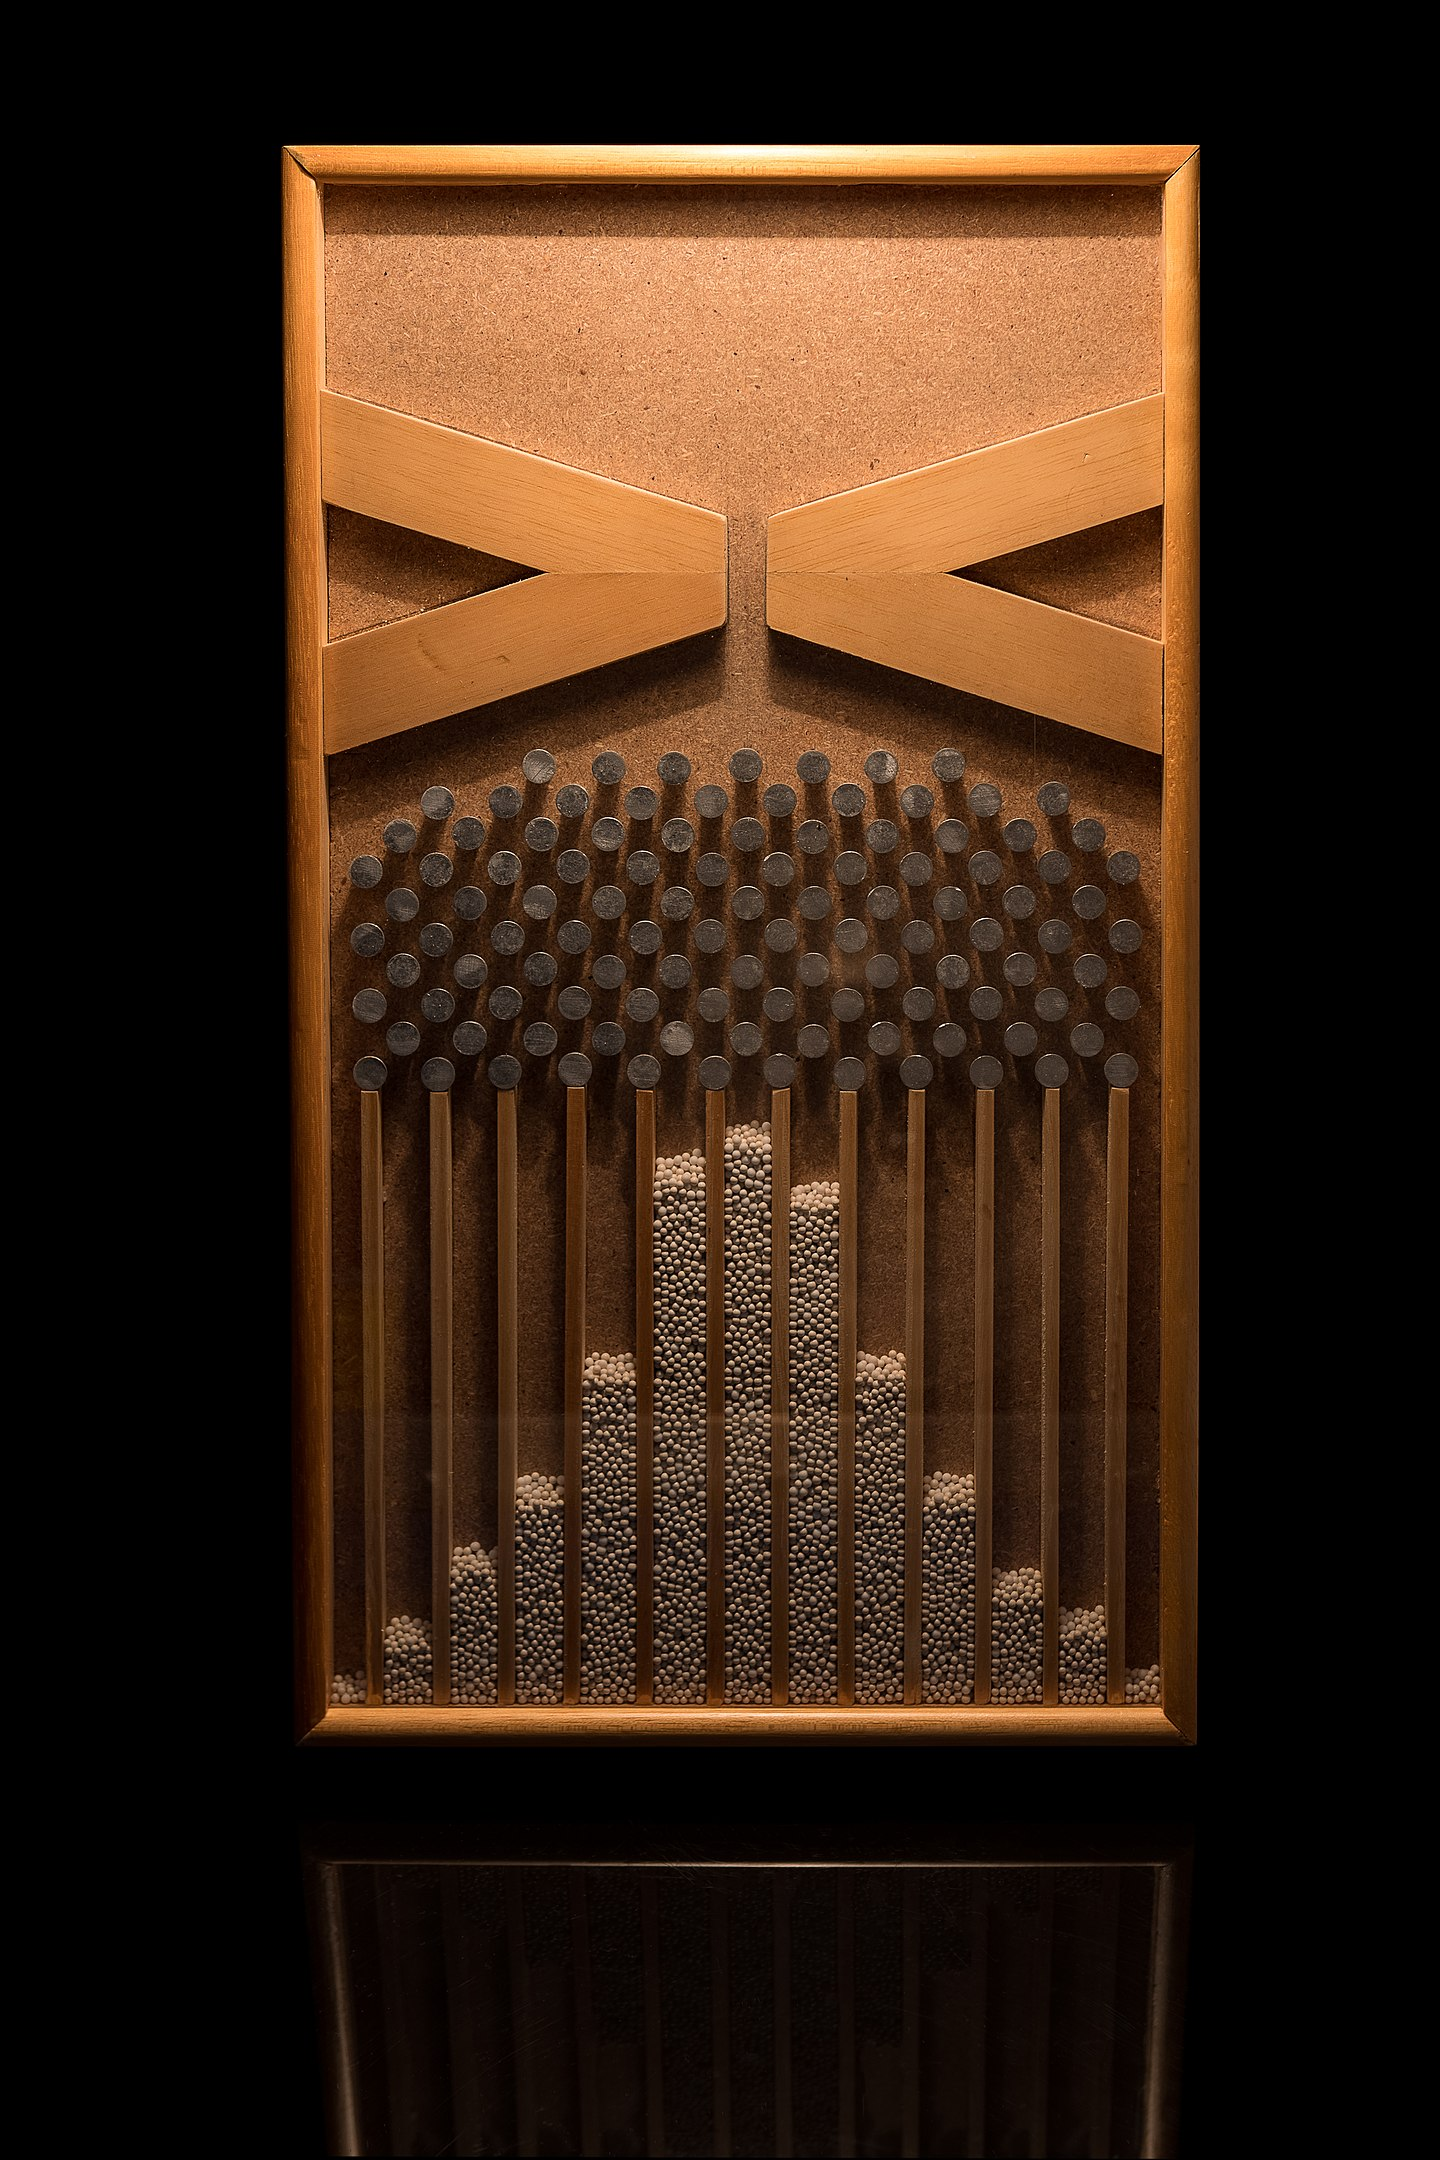
\includegraphics[width = 4cm]{text/FisherInformation/plots/GaltonBoard.jpg}
	\caption{This figure shows a picture of a Galton board. Taken from \cite{GaltonBoardPicture}.}
	\label{fig:GaltonPicture}
\end{figure}
It's a famous mechanical model that visualizes binomial distributions, which are approximations of the normal distribution. If we place many balls at the top of the board and let them fall to the bottom, the amount of balls that end up in each cell are distributed according to the binomial distribution. In this case, $x_i$ could assume the slot number which a ball can fall into. The $i$ could label multiple throws into the board, but for now we'll assume that there is only one experiment $i$. To introduce a parameter that influences the distribution of balls, let's say one can throw from different spots above the Galton board which we now control with the the value of $\theta$. For a known $\theta$, the resulting value of the statistical model represents the probability distribution $f(x_i|\theta) = p_\theta(x_i)$ for the probability of the different $x_i$ outcomes. A visual representation of the probability distributions for different $\theta$ can be seen in \cref{fig:GaltonDistributions}.
\begin{figure}
	\centering
	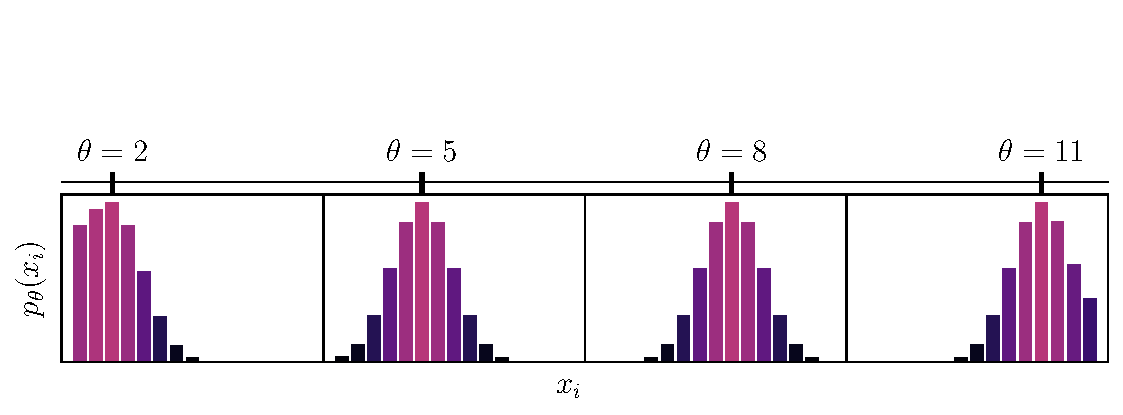
\includegraphics[width = \textwidth, clip, trim= 0cm 0cm 0cm 2.3cm]{text/FisherInformation/plots/GaltonDistributionsPlot.pdf}
	\caption{This figure shows the probability distributions for a Galton boards with different drop-in positions. The slots where the ball can end up are labeled by the value of $x_i$.}
	\label{fig:GaltonDistributions}
\end{figure}\\
In general, the statistical models might be more complex, where $\theta$ contains several parameters, $x$ being an element of a mathematical space other than $\mathbb{R}$ and the index $i$ denoting various different experiments, all depending on the same parameter, but having different possible outcomes and probability distributions.\\
What's of interest for the FI are cases where the parameters are not known before conducting the experiment, and have to be approximated by the different outcomes $x_i$.\\

Before we introduce the FI, let's look at an example from \cite{StatisticFisherInfoTutorial}. Let's consider a biased coin where we denote the probability of heads ($x_i = 1$) with $\theta$ and the probability of tails ($x_i = 0$) with $1-\theta$. We will now take a look at the outcome of $n$ tosses, represented by the variable $X^n$. For example, an observed result for $X^5$ could be $x^5 = (1,1,0,1,0)$. Let's consider another variable $Y$, whose observation is the sum of the total head throws $y = \sum x^n$. In our example case of $x^5 = (1,1,0,1,0)$, this would result in a value of $y = 3$. The probability for this variable $y$ is distributed according to the binomial distribution $f(y|\theta) = \binom{n}{y}\theta^y (1-\theta)^{n-y}$. Here the binomial coefficient $\binom{n}{y}$ represents the different combinations that result in the same value of $y$. This is needed because there are $2^n$ different possibilities for $x$, while there are only $n$ different possibilities for $y$.\\
If we now fix the outcome of $y$ and look at the conditional probability for the different $x^n$ that could have resulted in that $y$ value, we get $p(x|y,\theta) = 1/ \binom{n}{y}$. With $p(x|y,\theta)$ we denote the probability depending on $x$ for fixed $y$ and $\theta$. Although the probability of $y$ and $x$ both depend on $\theta$, the probability for $x$ when $y$ is fixed doesn't. After measuring $y$ there is no information about $\theta$ left in the measurement of $x$. This means that $y$ is fully descriptive of or "sufficient for" the parameter $\theta$. Measuring $y$ results in the same amount of information about the parameter $\theta$ as measuring the whole observation $x$. To quantify how much information a certain function of outputs $t(x)$, which is $y(x^n)$ in our example, contains about the parameters $\theta$, Fisher introduced the Fisher information.\\
The Fisher information is defined as 
\begin{equation}\label{eq:FIDefinition}
	I_{X,ij}(\theta) = \underset{x\in X}{E} \left[\tAbl{}{\theta_i}\log f(x|\theta) \cdot \tAbl{}{\theta_j}\log f(x|\theta)\right],
\end{equation}
where we used the expectation $E$
\begin{equation}
	\underset{x\in X}{E} \left[A(x)\right] = 
	\begin{cases}
		\sum_{x\in X} \left(A(x) p(x)\right) &\text{if $X$ is discrete},\\
		\int_{x\in X} A(x) p(x) \mathrm{d}x &\text{if $X$ is continuous}.
	\end{cases}
\end{equation}
Since the Fisher information is dependent of $\theta$, we can assume the value of $\theta$ to be fixed during calculation, which makes $f(x|\theta)$ equal to the probability density $p_\theta(x)$.\\ 
For $n$ independent experiments $X^n$, where $f(x^n|\theta) = \prod_{i=1}^n f(x_i|\theta)$, one can split the FI into 
\begin{equation}\label{eq:FIforIndependentExperiments}
	I_{X^n,ij}(\theta) = \prod_{i=1}^n I_{X_i,ij}(\theta).
\end{equation}
A proof of this can be found in \cref{sec:ProofFIforIndependentExperiments}.\\
For our example the FI yields $I_{X^n}(\theta) = I_{Y}(\theta) = n/(\theta(1-\theta))$\cite{StatisticFisherInfoTutorial}. This means that there is as much information about the $\theta$ contained in the measurement of $Y$ as in the measurement of $X^n$, which coincides with $Y$ being a sufficient measurement for $\theta$. \\
To give another example of how the FI represents the information obtainable about a parameter from a measurement, let's consider the family of normal distributions
\begin{equation}
	\mathcal{N}(x|\mu,\sigma) = \frac{1}{\sqrt{2\pi\sigma^2}}\mathrm{e}^{-(x-\mu)^2/(2\sigma^2)}.
\end{equation} 
These will now act as our statistical model $p_\theta(x) = \mathcal{N}(x|\theta)$ where $\theta = \{\theta_1,\theta_2\} = \{\mu, \sigma\}$. An observation would consist of a resulting value $x\in \mathbb{R}$, with it's probability distributed according to the statistical model. The FI from equation \cref{eq:FIDefinition} can be derived as 
\begin{equation}
	I(\mu,\sigma) = \frac{1}{\sigma^2}
	\begin{pmatrix}
		1 & 0 \\
		0 & 2
	\end{pmatrix}.
\end{equation}
We can now interpret the diagonal elements as measures of how much information a measurement contains about the corresponding parameter, and the off-diagonal elements as measurements of how similar the model changes when varying the corresponding parameters. To give a specific example, let's look at the diagonal component corresponding to $\mu$, $I_{11}(\mu,\sigma) = 1/\sigma^2$. This value indicates that for smaller $\sigma$, random values drawn from the distribution contain more information about $\mu$ than samples drawn from distributions with larger $\sigma$. For a visual guide, consider \cref{fig:NormalDistributionExample}.
\begin{figure}
	\centering
	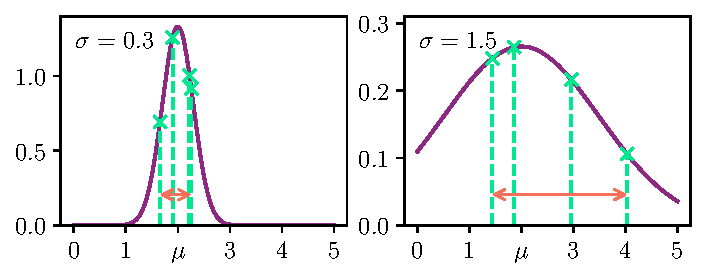
\includegraphics{"text/FisherInformation/plots/NormalDistributionPlot.pdf"}
	\caption{This figure shows two normal distributions centered around $\mu = 2$ with varying $\sigma$ parameters. It also shows 4 samples chosen randomly according to the distribution. It's visible that for the case of a smaller variance $\sigma$, the points tend to be closer to the center and also less spread apart, which makes the information about $\mu$ contained in a measurement larger for a smaller variance.}
	\label{fig:NormalDistributionExample}
\end{figure}
It can be seen that the smaller value of $\sigma$ results in a narrower spread of randomly drawn values, as indicated by the orange arrow. The values also tend to be closer to the mean value $\mu$ the smaller the variance $\sigma$ is. Therefore, if we had to predict the value of $\mu$ from knowing only a few drawn samples, it would be easier to use the values drawn from the distribution with the smaller variance, because the information contained in the samples, measured by the FI, is greater there. Keep in mind that all of these drawn values are randomly distributed. Therefore it is also possible to have two sets of random samples where the samples from the larger variance are better at predicting $\mu$, but statistically speaking the smaller variance tends to perform better.

To conclude this chapter, the Fisher information is used in statistics to measure the amount of information one can gather about a parameter $\theta$ by measuring the outcome of a probability distribution $p_\theta(x_i)$. It is defined in equation \cref{eq:FIDefinition}.

	
	
	\chapter{Neural Tangent Kernel}
	%This chapter introduces the \textbf{Neural Tangent Kernel} (NTK). While the Fisher Information describes the parameter derivative correlations of the loss functions, the NTK describes the similarities in the neural network output regarding the parameters.\\
\cref{sec:NTKderivation} presents a derivation of the NTK using the Gradient Flow assumption. \cref{sec:NTKInterpretation} provides further explanations on why the NTK arises in this context and how it can be interpreted.
	\section{Derivation from Gradient Flow}
	\subsection{What we call time}
A simple and intuitive way to introduce the NTK is via "\textbf{Gradient Flow}", which is an assumption related to the GD algorithm from \cref{sec:NetworkOptimization}. To quickly recap the update step from stochastic gradient descent, it is defined as 
\begin{equation}
	\theta' = \theta - \eta \nabla_\theta \mathscr{L}\left( \{(f_\theta(\mathbf{x}_i), \mathbf{y}_i)\}_{i=1}^{N} \right).
\end{equation}
The "flow" aspect arises when we start to ignore the discrete nature of these update steps and assume that the $\theta$ parameters change continuously. A visual demonstration of how this changes the evolution of the parameters can be seen in \cref{fig:GradientFlowPlot}. Here, the dashed markers represent the evolution under regular GD, while the solid line represents the evolution for gradient flow.
\begin{figure}
	\centering
	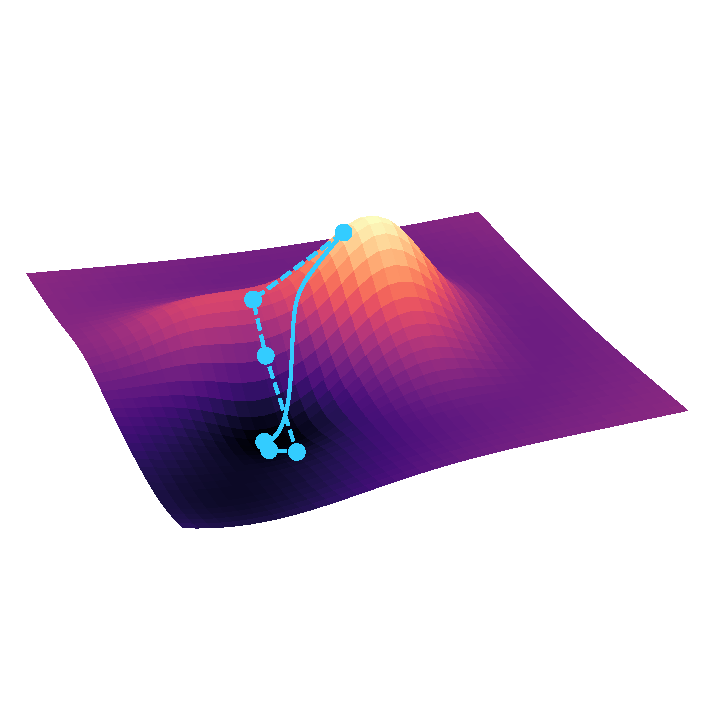
\includegraphics[width=12cm, clip, trim = 0cm 2.3cm 0cm 3.5cm]{text/NTK/GradientFlowPlot.pdf}
	\caption{This graph shows the effect of assuming gradient flow. The dashed line along with the circle markers show the positions during regular GD with finite step sizes, the solid line shows the path of the parameters under gradient flow.}
	\label{fig:GradientFlowPlot}
\end{figure}
To do this, we first introduce a notion of "time" into our system. We try to visualize the optimization process as an evolution of our parameters $\theta$ through this variable called time, which converts updating the parameters into moving further along the timeline of our parameters. We translate $\theta \rightarrow \theta(t)$ and $\theta' \rightarrow \theta(t+\Delta t)$. This time in our system doesn't work exactly the same way as physical time, but since the process of calculating better parameters and changing them is always associated with the expenditure of physical time, it is intuitive to refer to our system's propagation variable as "time". \\
Returning to the GD algorithm, since the learning rate $\eta$ affects the size of our update step, we will refer to $\eta$ as the amount of time it takes to update a parameter $\theta' \rightarrow \theta(t+\eta)$. The whole GD algorithm then becomes
\begin{equation}
	\theta(t+\eta) = \theta(t) - \eta \nabla_{\theta(t)} \mathscr{L}\left( \{(f_{\theta(t)}(\mathbf{x}_i), \mathbf{y}_i)\}_{i=1}^{N} \right)
\end{equation}
which we can rewrite to 
\begin{equation}
	\frac{\theta(t+\eta)-\theta(t)}{\eta} = - \nabla_{\theta(t)} \mathscr{L}\left( \{(f_{\theta(t)}(\mathbf{x}_i), \mathbf{y}_i)\}_{i=1}^{N} \right).
\end{equation}
When observing the term on the left side, readers who are familiar with calculus might recognize that it looks similar to the definition of a derivative in time
\begin{equation}
	\tAbl{}{t}\theta(t) = \lim_{\eta\rightarrow0} \frac{\theta(t+\eta)-\theta(t)}{\eta}.
\end{equation}
This means that for very small learning rates we can approximate the GD as 
\begin{equation}\label{eq:NTKThetaDerivative}
	\tAbl{}{t}\theta(t) = - \nabla_{\theta(t)} \mathscr{L}\left( \{(f_{\theta(t)}(\mathbf{x}_i), \mathbf{y}_i)\}_{i=1}^{N} \right)
\end{equation}
with the partial derivative of $\theta$ along the assumed time variable.\\
For visual simplicity reasons, let's define the $j$-th component of the network output for the $i$-th input point $f_{\theta(t)}(\mathbf{x}_i)_j$ as $F_{ij}$ and assume Einstein summation for the rest of the chapter.
This means that when an index is occuring twice, we don't denote a hidden summation over all possible values for this index (for example $a_kb_k = \sum_k a_kb_k$).\\
Because it will be convenient later, we also spell out one component of the $\nabla_\theta$ derivation of the loss function further by using the chain rule as
\begin{align}
	\tAbl{\theta_k}{t} &= - \tAbl{}{\theta_k}\mathscr{L}\left( \{(f_{\theta(t)}(\mathbf{x}_i), \mathbf{y}_i)\}_{i=1}^{N} \right)\nonumber\\
	&= - \pAbl{\mathscr{L}}{F_{ij}} \cdot \tAbl{F_{ij}}{\theta_k}.
\end{align} 

\subsection{Derivation of the NTK}
This notion of time affects not only the parameters, but also everything that depends on them. For example, since the network output of a fixed architecture for a given input data point only depends on the parameters of the network, it can also be mathematically viewed as dependent on the time $f_{\theta}(\mathbf{x}_i) \rightarrow f_{\theta(t)}(\mathbf{x}_i)$. This means we can also calculate the derivative of one of the network outputs $f_{\theta(t)}(\mathbf{x}_i)_j = F_{ij}$ to
\begin{align}
	\tAbl{}{t} F_{ij} &= \pAbl{F_{ij}}{\theta_k}\tAbl{\theta_k}{t}\nonumber\\
	&= \pAbl{F_{ij}}{\theta_k} \left(- \pAbl{\mathscr{L}}{F_{ij}} \tAbl{F_{ij}}{\theta_k} \right)\label{eq:NTKarisesFromHere}\\
	&= - \underbrace{\pAbl{F_{ij}}{\theta_k} \pAbl{F_{lm}}{\theta_k}}_\mathlarger{=\vcentcolon \Lambda_{iljm}}
	\pAbl{\mathscr{L}}{F_{lm}}.\nonumber
\end{align}
In the last line, we used the fact that $F_{ij}$ only depend explicitly on $\theta$, which means that the total and partial derivative ar interchangeable.
The rank 4 hypermatrix $\Lambda$ is what we call the Neural Tangent Kernel for GD. We sorted the indices of this matrix so that the first two refer to the input points of $f$ and the last two refer to the components of the output dimensions of the neural network. Note that this NTK is derived directly from the update algorithm of the GD for infinitely small $\eta$, the equations above don't hold for other optimization systems.\\
Another way to derive the NTK using an approximation of $\Delta \mathscr{L}$ for small $\eta$ can be seen around page 196 of \cite{ThePrinciplesOfDeepLearningTheory}. The NTK derived there also works for tensorial gradient descent with a learning rate tensor $\eta_{ij}$.
	\section{Interpretation}
	Through \cref{eq:NTKarisesFromHere} the NTK is defined as 
\begin{equation}\label{eq:NTKDefinition}
	\Lambda_{i,j,\alpha,\beta} = \nabla_\theta f_\theta(\mathbf{x}_i)_\alpha \cdot \nabla_\theta f_\theta(\mathbf{x}_j)_\beta.
\end{equation}
For now, let's assume that the neural network has only one output $f_\theta(\mathbf{x}_i)_\alpha \rightarrow f_\theta(\mathbf{x}_i)$, which gets rid of the $\alpha$ and $\beta$ indices for us and makes the NTK a regular matrix. We can use this matrix to calculate the "time" derivative of the neural network output similar to \cref{eq:NTKarisesFromHere} by 
\begin{equation}\label{eq:NTKExplanation}
	\pAbl{}{t}f_{\theta(t)}(\mathbf{x}_i) = \sum_j \Lambda_{i,j} \left(- \pAbl{\mathscr{L}}{f_{\theta(t)}(\mathbf{x}_j)}\right).
\end{equation}
This means that the evolution of the network output for input $\mathbf{x}_i$ is influenced by the outputs for other input values $\mathbf{x}_j$ through the NTK. We can investigate this further by taking a look at the definition of the NTK above in \cref{eq:NTKDefinition}. \\
A mathematical kernel $K$ is defined as a function
\begin{equation}
	K(\mathbf{x}_i, \mathbf{x}_j) = \phi(\mathbf{x}_i)\cdot\phi(\mathbf{x}_i),
\end{equation}
with another so-called "feature map" function $\phi$ that maps the points $\mathbf{x}_i$ into a higher dimensional inner product space called the "feature space". The kernel $K$ assigns a scalar value to the two points by comparing their "features" via a scalar product in the feature space. For more specific information on Kernels and how they are used, please refer to \cite{KernelMethod}.\\
In our case the feature map is $\nabla_\theta$ which maps our scalar network output onto a vector that contains the derivatives of the network output with respect to all of the various parameters. This is our feature space, because what we're interested in is how moving in $\theta$ space changes the output values of our network. If we compare those two mappings we get a value that measures how closely the direction that increases $f_\theta(\mathbf{x}_i)$ in the most effective way matches with the direction that increases $f_\theta(\mathbf{x}_j)$ most effectively  (which are the directions the gradients points to). For example, $\Lambda_{i,j}=0$ means that varying $\theta$ in the direction that changes $f_\theta(\mathbf{x}_i)$ most effectively results in 0 change for $f_\theta(\mathbf{x}_j)$.\\

Coming back to \cref{eq:NTKExplanation} the right side is the negative loss derivative with respect to $f_\theta(\mathbf{x}_j)$. Since we update the parameters in a way that minimizes the loss most effectively in gradient flow, the negative loss derivative with respect to $f_\theta(\mathbf{x}_j)$ describes how beneficial increasing $f_\theta(\mathbf{x}_j)$ is for our system. If we now multiply this with the NTK, which is a kernel that describes how similar $f_\theta(\mathbf{x}_i)$ and $f_\theta(\mathbf{x}_j)$ behave when changing theta, and sum everything up, we get the change of the function value $f_\theta(\mathbf{x}_i)$ as result.\\
In $\theta$ space, we can directly relate the evolution of $\theta$ to its negative loss derivative, because the parameters themselves are what we update with our algorithm. For the derivative of the output values we need the NTK as well, because we don't change the output values directly. If the loss derivative with respect to an output value tells the system that it \textit{should increase this output value}, the system \textit{changes the parameters} in a way that increases this output value. The difference to the derivative of $\theta$ is that the change of parameters now doesn't reflect in just one output, but in every other output value as well. That's where the NTK arises in the equation. The NTK is, in a way, a translation of the SGD into the space of outputs of the neural network.\\
All of the explanations above apply to the 4 dimensional hypermatrix form of the NTK for multidimensional neural network output as well, which can be seen when comparing \cref{eq:NTKExplanation} to \cref{eq:NTKarisesFromHere}.
	
	
	
	\nocite{*}
	\printbibliography[title=Literature]
	\begin{appendices}
		\chapter{Appendix Example}
	\end{appendices}
	
\end{document}